%% Submissions for peer-review must enable line-numbering
%% using the lineno option in the \documentclass command.
%%
%% Preprints and camera-ready submissions do not need
%% line numbers, and should have this option removed.
%%
%% Please note that the line numbering option requires
%% version 1.1 or newer of the wlpeerj.cls file, and
%% the corresponding author info requires v1.2

\documentclass[fleqn,10pt,lineno]{wlpeerj} % for journal submissions

% ZNK -- Adding headers for pandoc

\setlength{\emergencystretch}{3em}
\providecommand{\tightlist}{
\setlength{\itemsep}{0pt}\setlength{\parskip}{0pt}}
\usepackage{lipsum}
\usepackage[unicode=true]{hyperref}
\usepackage{longtable}



\usepackage{lipsum}

\title{xxx}

\author[1, 2]{Tobias Roth}

\corrauthor[1, 2]{Tobias Roth}{\href{mailto:t.roth@unibas.ch}{\nolinkurl{t.roth@unibas.ch}}}
\author[2]{Lukas Kohli}


\affil[1]{Zoological Institute, University of Basel, Basel, Switzerland}
\affil[2]{Hintermann Weber AG, Austrasse 2a, 4153 Reinach, Switzerland}


%
% \author[1]{First Author}
% \author[2]{Second Author}
% \affil[1]{Address of first author}
% \affil[2]{Address of second author}
% \corrauthor[1]{First Author}{f.author@email.com}

% 

\begin{abstract}
xxx
% Dummy abstract text. Dummy abstract text. Dummy abstract text. Dummy abstract text. Dummy abstract text. Dummy abstract text. Dummy abstract text. Dummy abstract text. Dummy abstract text. Dummy abstract text. Dummy abstract text.
\end{abstract}

\begin{document}

\flushbottom
\maketitle
\thispagestyle{empty}

\begin{verbatim}
## Warning: package 'kableExtra' was built under R version 3.4.4
\end{verbatim}

\section*{Introduction}\label{introduction}
\addcontentsline{toc}{section}{Introduction}

\section*{Materials \& Methods}\label{materials-methods}
\addcontentsline{toc}{section}{Materials \& Methods}

\subsection*{Monitoring data}\label{monitoring-data}
\addcontentsline{toc}{subsection}{Monitoring data}

\begin{itemize}
\tightlist
\item
  Selection of sample sites based on 1366 K\_Standort.csv column
  ``E23\_1366''.
\item
  Three surveys 2003-2007, 2008-2012 and 2013 - 2017.
\end{itemize}

\subsection*{Plant traits}\label{plant-traits}
\addcontentsline{toc}{subsection}{Plant traits}

Functional traits:

\begin{itemize}
\tightlist
\item
  SLA: specific leaf area
\item
  CH: canopy height
\item
  SM: Seed mass
\end{itemize}

Ellenberg indicator values:

\begin{itemize}
\tightlist
\item
  L: light
\item
  N: Nutrient contentent
\item
  T: Temperature
\item
  F: Huminity
\end{itemize}

Community measures:

\begin{itemize}
\tightlist
\item
  Species richness: number of recorded species per \(10m^2\).
\item
  Spatial turnover (beta-diversity): Average turnover between all
  pair-wise combinations of study plots.
\item
  gamma diversity: Total number of species recorded in all study plots.
\end{itemize}

\subsubsection{Community measures}\label{community-measures}

The temporal turnover (i.e.~species exchange ratio sensu Hillebrand et
al. (2018)) is the proportion of species that differ between two time
points calculated as

\(\text{Spatial turnover} = \frac{\text{Species gained} + \text{Species lost}}{\text{Total species observed in both timepoints}}\).

\subsection*{Statistical analyses}\label{statistical-analyses}
\addcontentsline{toc}{subsection}{Statistical analyses}

Environmental variables were standardized.

\section*{Results}\label{results}
\addcontentsline{toc}{section}{Results}

\begin{table}[ht]
\centering
\begin{tabular}{lrrrrr}
  \hline
Measures & Period 1 & Period 2 & Period 3 & Temporal-Trend & P-value \\ 
  \hline
Alpha-diversity & 46.36 & 46.72 & 46.45 & 0.002 & 0.896 \\ 
  Beta-diversity & 0.68 & 0.65 & 0.65 &  &  \\ 
  Gamma-Diversity & 517 & 529 & 517 &  &  \\ 
  Temperature value & 3.12 & 3.14 & 3.14 & 0.013 & 0.060 \\ 
  Huminity value & 2.99 & 2.98 & 2.99 & 0.006 & 0.405 \\ 
  Nutrients value & 3.22 & 3.22 & 3.22 & -0.004 & 0.698 \\ 
  Light value & 3.57 & 3.56 & 3.56 & -0.010 & 0.196 \\ 
  Canopy height & -1.24 & -1.22 & -1.23 & 0.013 & 0.307 \\ 
  Specific leaf area & 8.21 & 8.27 & 8.24 & 0.030 & 0.621 \\ 
  Seed mass & -0.34 & -0.32 & -0.33 & 0.010 & 0.596 \\ 
   \hline
\end{tabular}
\caption{Average measures of community structure for the three survey periods (in each period all sites are surveyed once). The temporal trends and p-values are based on linear mixed models with normal distribution (except for alpha-diversity with Poisson distribution) with site-ID as random effect. Temporal-trends are given per 10 years. Linear mixed models could not be applied for beta- and gamma-diversity because measures are not available for the single sites.} 
\label{temporaltrends}
\end{table}

The different measures of total community structure suggested that plant
communities of mountain hay meadow were stable between 2003 and 2017
(Table \ref{temporaltrends}): for each of the three 5-year survey
periods the averages of alpha-, beta- and gamma-diversity, average
Ellenberg values for temperature, nutrients, light and huminity, and
average of species' canopy height, specific leaf area and seed mass did
not vary much among the three sampling periods. For all measures, the
average temperal trend per site did not differ significantly from a
constant trend. Note that beta- and gamma-diversity are note available
for single sites and thus mixed models to calculate the p-value could
not be applied.

The temporal stability as inferred from the community measures were,
however, in contrast to the large temporal turnover of recorded species.
The percentage \(\pm\) SD of species that differ between the first and
second survey at a site was 37.55 \(\pm\) 10.46 and the percentage of
species that differ between the second and third survey was 35.63
\(\pm\) 10.33. The decrease in the temporal turnover between the first
and second survey to the temporal turnover between the second and third
survey was statistically significant (Binomial generalized linear model;
effect size = -0.078; p = 0.027).

This spatial turnover might be partly explained by species that remained
undetected in one of the surveys, but it might also be the result of
species that newly colonized sites (species gains) and species that
truely disappeared from sites (species losses). Spatial turnover will be
high if the probability a site is colonized by a species is high
(i.e.~high colonization probability) and/or if the probability that a
species survives at a site between two time points is low (i.e.~low
local survival). We found that the variation in local survival and
colonization, was largely due to differences between species and only to
a lesser extend to the differences between locations: while the variance
of the species random effect in a binomial linear mixed model for local
survival was about 4.46 times larger than the variance of the sampling
site random effect, in the model for colonization the variance among
species was even 9.15 times bigger than the variance among sites.

\begin{table}

\caption{\label{tab:resdifeffects}Comparision of results from different drivers to explain colonization probability (a) and local survvival (b). See methods for the tested models.}
\centering
\begin{tabular}[t]{lrrr}
\toprule
Model & Df & AIC & Delta-AIC\\
\midrule
\addlinespace[0.3em]
\multicolumn{4}{l}{\textit{(a) Colonization probability}}\\
\hspace{1em}Temperature driven & 6 & 19321.85 & 0.00\\
\hspace{1em}Nitrogen driven & 6 & 19691.81 & 369.96\\
\hspace{1em}Precipitation driven & 6 & 20032.57 & 710.73\\
\hspace{1em}Random change & 3 & 20038.36 & 716.52\\
\hspace{1em}Land-use driven & 6 & 20041.22 & 719.38\\
\addlinespace[0.3em]
\multicolumn{4}{l}{\textit{(b) Local survival probability}}\\
\hspace{1em}Temperature driven & 6 & 9811.08 & 0.00\\
\hspace{1em}Nitrogen driven & 6 & 9827.78 & 16.70\\
\hspace{1em}Land-use driven & 6 & 9834.31 & 23.23\\
\hspace{1em}Random change & 3 & 9837.76 & 26.68\\
\hspace{1em}Precipitation driven & 6 & 9838.55 & 27.47\\
\bottomrule
\end{tabular}
\end{table}

We thus inferred if we could explain differences in colonization
probability and local survival with Ellengerg species values for
temperature, humidity, nutrient or light. We found that both
colonization probability and local survival probability was best
explained by temperature (i.e.~highest colonization or local survival
probability of species with an Ellenberg value for Temperature that
corresponds to the annual average temperature of the site) followed by
nutrient availability (i.e.~highest colonization or local survival
probability of species with an Ellenberg value for nutrient availability
that corresponds to the annual N deposition rate estimated for the site;
Table \ref{tab:resdifeffects}).

\begin{figure}
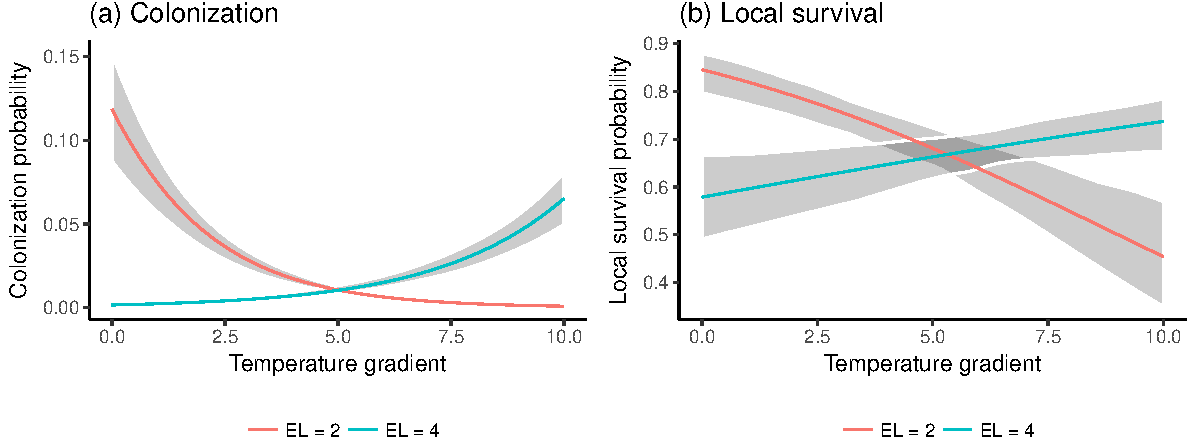
\includegraphics[width=1\linewidth]{Manuscript_files/figure-latex/Teff-1} \caption{Colonization (a) and local survival (b) of low temperature species (Ellenberg T = 2; red line) and high temperature species (Ellengerg T = 4) species along the temperature gradient. Given are means and 95\%-Credible Intervals from logistic linear mixed models.}\label{fig:Teff}
\end{figure}

\begin{figure}
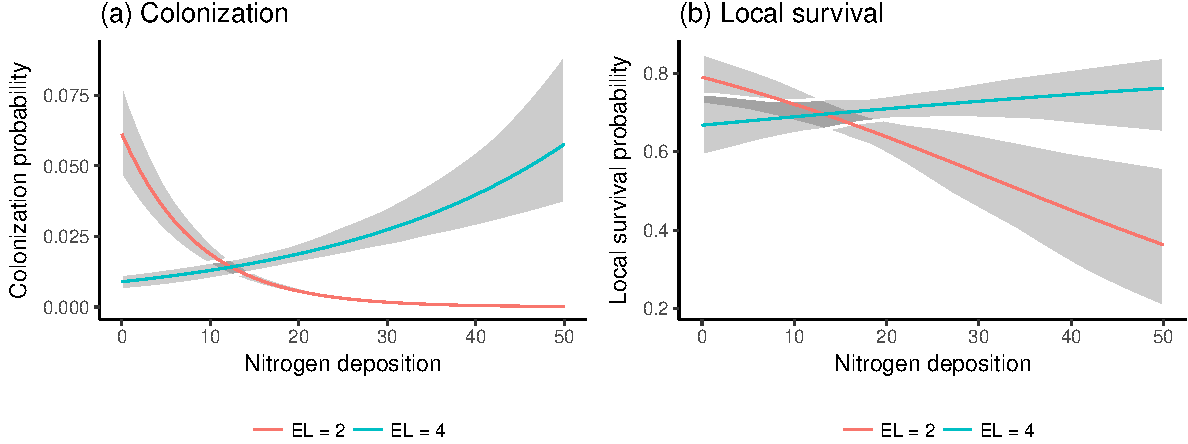
\includegraphics[width=1\linewidth]{Manuscript_files/figure-latex/Neff-1} \caption{Colonization (a) and local survival (b) of oligotrophic (Ellenberg N = 2; red line) and eutrophic (Ellengerg N = 4) species along the N deposition gradient. Given are means and 95\%-Credible Intervals from logistic linear mixed models.}\label{fig:Neff}
\end{figure}

While the colonization and local survival probability of cold living
species (Ellenberg T = 2) declindes along the temperature gradient, the
colonization and local survival probability of warm living species
(Ellenberg T = 4) increases along the temperature gradient (Fig.
\ref{fig:Teff}). Similarly for nutrient values: while the colonization
and local survival probability of oligotrophic species (Ellenberg N = 2)
declindes along the N deposition gradient, the colonization and local
survival probability of eutrophic species (N = 4) increases along the N
deposition gradient (Fig. \ref{fig:Neff}).

For the temperature driven and nitrogen driven models in table
\ref{tab:resdifeffects} we also tested whether the strength of the
effects differed from the first/second to the second/third survey
period. For the temperatur driven models we found that the differences
how species with different Ellenberg T values responded to the average
annual temperature of a site tended to decrease from the first/second
study period to the second/third study period (colonization probability:
period x Ellenberg T x annual mean temperature of site = -0.0098, p =
0.70; local survival: period x Ellenberg T x annual mean temperature of
site = -0.072, p = 0.051). In contrast, however, the differences how
species with different Ellenberg N values responded to the average N
deposition of a site tended to increase from the first/second study
period to the second/third study period (colonization probability:
period x Ellenberg N x N deposition at site = 0.025, p = 0.74; local
survival: period x Ellenberg N x N deposition at site = 0.075, p =
0.50).

\begin{figure}
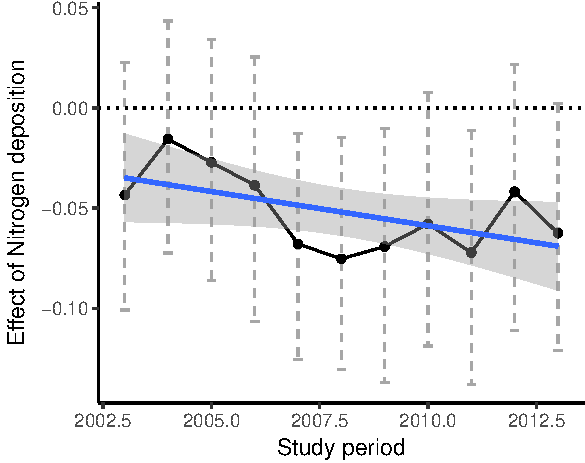
\includegraphics[width=1\linewidth]{Manuscript_files/figure-latex/figconsequences-1} \caption{Beschreibung einfügen.}\label{fig:figconsequences}
\end{figure}

It thus seems that temperature is the main driver of species turnover in
the first part of the study period and its importance is slightly
decreasing over time and nitrogen deposition becomes relatively more
important as a driver that shapes the species communities. We thus
expect to see that the correlation of the mean temperature value of a
community with the yearly annual temperature of the site (temperature
correlation) is decreasing over the years while the correlation of the
mean nutrient value of a community with the N deposition of the site
(nitrogen correlation) is increasing over the years. Our results tent to
be in line with this expectation (linear model: temporal trend of
temperature correlation x temporal trend of nitrogen correlation =
-0.0015, p = 0.067), however the change in the correlation over the
study period remained week and the temperature correlation remained
stronger than the nitrogen correlation over the entire study period
(Left panel of Fig. \ref{fig:figconsequences}). More important, however,
was the effect on our model that we used to infer whether and how strong
the spatial variation in N deposition is correlated with Nitrogen
deposition. If we apply that model the estimated effect of N depositon
on total species richness is increasing over the study period (right
panel of \ref{fig:figconsequences}).

\section*{Discussion}\label{discussion}
\addcontentsline{toc}{section}{Discussion}

\begin{itemize}
\item
  Any empty space that could be caused by any disturbance that let to
  the local disappearance of species is likely to be fiellied by
  eutrophic species. Disturbance depends on the site, while colonization
  depends on species characteristics.
\item
  Altough N deposition considerabely declinded between 2005 and 2015, we
  could not detect major shifts in plant community structure during the
  same time period.
\item
  Eutrophic species have rather high local survival across the entire
  deposition gradient, while oligotrophic species have much reduced
  local survival at high N deposition. This suggests that it takes much
  more time to replace eutrophic by oligotrophic species than replacing
  oligotrophic by eutrophic species.
\item
  Our data on colonization and local survival (i.e.~temporal variation)
  confirm the empirical critical loads that we infered from anlysing
  spatial co-variation of N deposition and species richness.
\item
  Local survival is higher for low temperature plants --\textgreater{}
  This could explain the decrease in cumminity change along elevation.
  This could also explain the differences at mount summets were space
  was empty in the beginning.
\item
  Climatic effects are more likely to be reversed thant effects due to
  fertilization.
\end{itemize}

\section*{Conclusions}\label{conclusions}
\addcontentsline{toc}{section}{Conclusions}

xxx

\section*{Acknowledgements}\label{acknowledgements}
\addcontentsline{toc}{section}{Acknowledgements}

xxx

\section*{References}\label{references}
\addcontentsline{toc}{section}{References}

\hypertarget{refs}{}
\hypertarget{ref-Hillebrand2018}{}
Hillebrand, Helmut, Bernd Blasius, Elizabeth T. Borer, Jonathan M.
Chase, John A. Downing, Britas Klemens Eriksson, Christopher T.
Filstrup, et al. 2018. ``Biodiversity Change Is Uncoupled from Species
Richness Trends: Consequences for Conservation and Monitoring.''
\emph{Journal of Applied Ecology} 55 (1): 169--84.
doi:\href{https://doi.org/10.1111/1365-2664.12959}{10.1111/1365-2664.12959}.



\end{document}
